\chapter{Содержание работы}
\textit{Цель работы}:  построение доверительных интервалов для математического ожидания и дисперсии нормальной случайной величины
\begin{enumerate}[wide=0pt]
	\item Для выборки объема n из генеральной совокупности X реализовать в виде программы на ЭВМ:
	\begin{enumerate}
		\item вычисление точечных оценок $\hat\mu(\vec X_n)$ и $S^2(\vec X_n)$ математического ожидания $MX$ и дисперсии $DX$ соответственно;
		\item вычисление нижней и верхней границ $\underline\mu(\vec X_n)$, $\overline\mu(\vec X_n)$ для $\gamma$-доверительного интервала для математического ожидания $MX$;
		\item вычисление оценок $\hat{\mu}$ и $S^2$ математического ожидания MX и дисперсии DX;
		\item вычисление нижней и верхней границ $\underline\sigma^2(\vec X_n)$, $\overline\sigma^2(\vec X_n)$ для $\gamma$-доверительного интервала для дисперсии $DX$;
	\end{enumerate}
	\item вычислить $\hat\mu$ и $S^2$ для выборки из индивидуального варианта;
	\item для заданного пользователем уровня доверия $\gamma$ и $N$ – объёма выборки из индивидуального варианта:
	\begin{enumerate}
		\item на координатной плоскости $Oyn$ построить прямую $y = \hat\mu(\vec{x_N})$, также графики функций $y = \hat\mu(\vec x_n)$, $y = \underline\mu(\vec x_n)$ и $y = \overline\mu(\vec x_n)$ как функций объема $n$ выборки, где $n$ изменяется от 1 до $N$;
		\item на другой координатной плоскости $Ozn$ построить прямую $z = S^2(\vec{x_N})$, также графики функций $z = S^2(\vec x_n)$, $z = \underline\sigma^2(\vec x_n)$ и $z = \overline\sigma^2(\vec x_n)$ как функций объема $n$ выборки, где $n$ изменяется от 1 до $N$.
	\end{enumerate}
\end{enumerate}

\chapter{Теоретические сведения}
Дана случайная величина X, закон распределения которой известен с точностью до неизвестного параметра $\theta$. 

\begin{definition}
Интервальной оценкой с коэффициентом доверия $\gamma$ ($\gamma$-доверительной интервальной оценкой) параметра $\theta$ называют пару статистик $\underline{\theta}(\vec X), \overline{\theta}(\vec X)$ таких, что

$$P\{\underline{\theta}(\vec X)< \theta< \overline{\theta}(\vec X)\}=\gamma$$ 
\end{definition}

Формулы для вычисления границ $\gamma$-доверительного интервала для математического ожидания:

\begin{equation}
	\begin{array}{cc}
		\underline\mu(\vec X_n)=\overline X - \cfrac{S(\vec X)t^{St(n-1)}_{\frac{1+\gamma}{2}}}{\sqrt{n}}\; ; & \overline\mu(\vec X_n)=\overline X + \cfrac{S(\vec X)t^{St(n-1)}_{\frac{1+\gamma}{2}}}{\sqrt{n}}
	\end{array}
\end{equation}

$\overline X$ -- точечная оценка математического ожидания;

$S^2(\vec X)$ -- точечная оценка дисперсии;

$n$ -- объем выборки;

$\gamma$ -- уровень доверия;

$t^{St(n-1)}_{\frac{1+\gamma}{2}}$ -- квантили соответствующих уровней распределения Стьюдента с n - 1 степенями свободы.

Формулы для вычисления границ $\gamma$-доверительного интервала для дисперсии:
\begin{equation}
	\begin{array}{cc}
		\underline\sigma(\vec X_n)= \cfrac{(n-1)S^2(\vec X)}{t^{\chi^2(n-1)}_{\frac{1+\gamma}{2}}};\; & \overline\sigma(\vec X_n)= \cfrac{(n-1)S^2(\vec X)}{t^{\chi^2(n-1)}_{\frac{1-\gamma}{2}}}
	\end{array}
\end{equation}

$S^2(\vec X)$ -- точечная оценка дисперсии;

$n$ -- объем выборки;

$\gamma$ -- уровень доверия;

$t^{\chi^2(n-1)}_{\frac{1+\gamma}{2}}$ -- квантили соответствующих уровней распределения $\chi^2(n-1)$ с n - 1 степенями свободы.


\chapter{Текст программы} 
\begin{lstlisting}
function main()
  pkg load statistics
  X = [-0.68, 0.71, 2.27, 0.38, 0.14, 0.06, 1.21, -0.59, 0.44, 1.98, 1.00, ...
     -0.88, -0.08, 1.87, -0.74, 0.83, -1.45, 0.58, 0.48, 3.26, 0.02, 0.26, ...
     2.96, 1.78, 0.58, 0.08, -1.60, 1.26, 1.28, -0.36, 0.15, -0.38, -1.04, ...
     0.95, -2.17, -0.30, 1.09, 0.39, 1.06, 0.98, -2.55, 2.62, -1.58, 3.75, ...
    -1.43, 0.92, 2.75, -0.55, 1.48, -0.96, 0.50, 2.67, -0.58, 0.41, -0.46, ...
    -0.48, 1.68, -0.08, 1.76, 0.08, -1.15, 0.66, 1.54, 0.17, -0.20, 1.34, ...
    1.08, 1.59, -0.05, 0.15, -0.35, 0.58, -0.87, 1.73, -0.27, 0.00, -0.67, ...
    0.13, 1.75, -0.59, 1.31, 1.20, 0.53, 0.14, -0.35, 1.00, -0.01, 0.21, ...
    1.58, -0.02, 1.28, 1.34, -1.66, 0.30, 0.08, 0.66, -0.26, 1.54, 1.22, ...
    1.24, 0.11, 0.79, -0.83, 1.41, 0.17, 0.55, 1.60, 1.26, 1.06, 0.39, ...
    -0.77, 1.49, 0.92, -1.58, 1.19, 0.13, 0.26, -2.14, 0.08, -1.75];

  gamma = 0.9;
  n = length(X);
  % Точечная оценка мат. ожидания
  mu = mean(X);
  % Точечная оценка дисперсии
  s2 = var(X);

  mu_low = get_mu_low(n, mu, s2, gamma);
  mu_high = get_mu_high(n, mu, s2, gamma);

  s2_low = get_s2_low(n, s2, gamma);
  s2_high = get_s2_high(n, s2, gamma);

  fprintf('a) Точечная оценка математического ожидания = %.3f\n', mu);
  fprintf('   Точечная оценка дисперсии = %.3f\n', s2);
  fprintf('б) Нижняя граница доверительного интервала для математического ожидания = %.3f\n', mu_low);
  fprintf('   Верхняя граница доверительного интервала для математического ожидания = %.3f\n', mu_high);
  fprintf('в) Нижняя граница доверительного интервала для дисперсии = %.3f\n', s2_low);
  fprintf('   Верхняя граница доверительного интервала для дисперсии = %.3f\n', s2_high);

  mus = zeros(1, n);
  s2s = zeros(1, n);

  mus_low = zeros(1, n);
  mus_high = zeros(1, n);
  s2s_low = zeros(1, n);
  s2s_high = zeros(1, n);

  for i = 1:n
    mu = mean(X(1:i));
    s2 = var(X(1:i));
    mus(i) = mu;
    s2s(i) = s2;
    mus_low(i) = get_mu_low(i, mu, s2, gamma);
    mus_high(i) = get_mu_high(i, mu, s2, gamma);
    s2s_low(i) = get_s2_low(i, s2, gamma);
    s2s_high(i) = get_s2_high(i, s2, gamma);
  end

  plot(1:n, [(zeros(1, n) + mu)', mus', mus_low', mus_high']);
  xlabel('n');
  ylabel('y');

  legend('точечная оценка \mu(x_N)', 'точечная оценка \mu(x_n)', 'верхняя граница ДО \mu', ...
    'нижняя граница ДО \mu', 'Interpreter', 'tex');
  figure;
  plot(1:n, [(zeros(1, n) + s2)', s2s', s2s_low', s2s_high']);
  xlabel('n');
  ylabel('z');
  legend('точечная оценка S^2(x_N)', 'точечная оценка S^2(x_n)', 'верхняя граница ДО \sigma', ...
      'нижняя граница ДО \sigma', 'Interpreter', 'tex');
end

function mu_low = get_mu_low(n, mu, s2, gamma)
  mu_low = mu - sqrt(s2) * tinv((1 + gamma) / 2, n - 1) / sqrt(n);
end

function mu_high = get_mu_high(n, mu, s2, gamma)
  mu_high = mu + sqrt(s2) * tinv((1 + gamma) / 2, n - 1) / sqrt(n);
end

function s2_low = get_s2_low(n, s2, gamma)
  s2_low = ((n - 1) * s2) / chi2inv((1 + gamma) / 2, n - 1);
end

function s2_high = get_s2_high(n, s2, gamma)
  s2_high = ((n - 1) * s2) / chi2inv((1 - gamma) / 2, n - 1);
end
\end{lstlisting}
\chapter{Результаты расчетов}
\begin{enumerate}
	\item Точечные оценки $\hat \mu (\vec x_n)$ и $ S^2 (\vec x_n)$ математического ожидания MX и дисперсии DX соответственно: $\hat \mu (\vec x_n) = 0.416$, $ S^2 (\vec x_n) = 1.340$
	\item Вычисление нижней и верхней границ $\underline \mu (\vec x_n)$, $\overline \mu (\vec x_n)$ для $\gamma$-доверительного интервала для математического ожидания DX: $\underline \mu (\vec x_n) = 0.592$, $\overline\mu (\vec x_n) = 0.241$
	
	\item Вычисление нижней и верхней границ $\underline \sigma (\vec x_n)$, $\overline \sigma (\vec x_n)$ для $\gamma$-доверительного интервала для математического ожидания MX: $\underline \sigma (\vec x_n) = 1.096$, $\overline \sigma (\vec x_n) = 1.682$
\end{enumerate}
%
\begin{figure}[H]
		\centering
		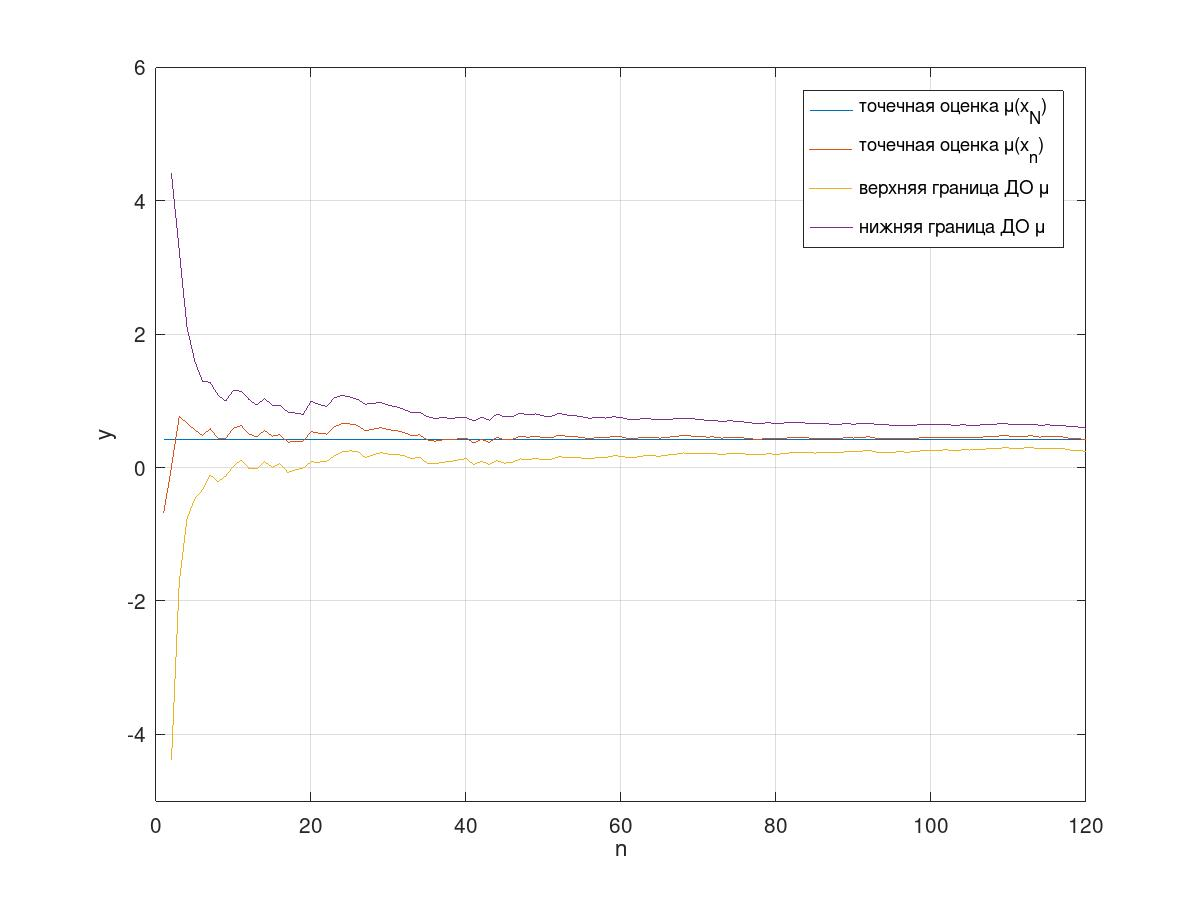
\includegraphics[scale=0.4]{assets/g-1.jpg}
		\caption{Прямая $y=\hat \mu (\vec x_N)$ и графики функций $y=\hat \mu (\vec x_n), y= \underline \mu (\vec x_n), y =\overline \mu (\vec x_n)$ как функций объема n выборки, где n изменяется от 1 до N.}
\end{figure}
%
\begin{figure}[H]
	\centering
	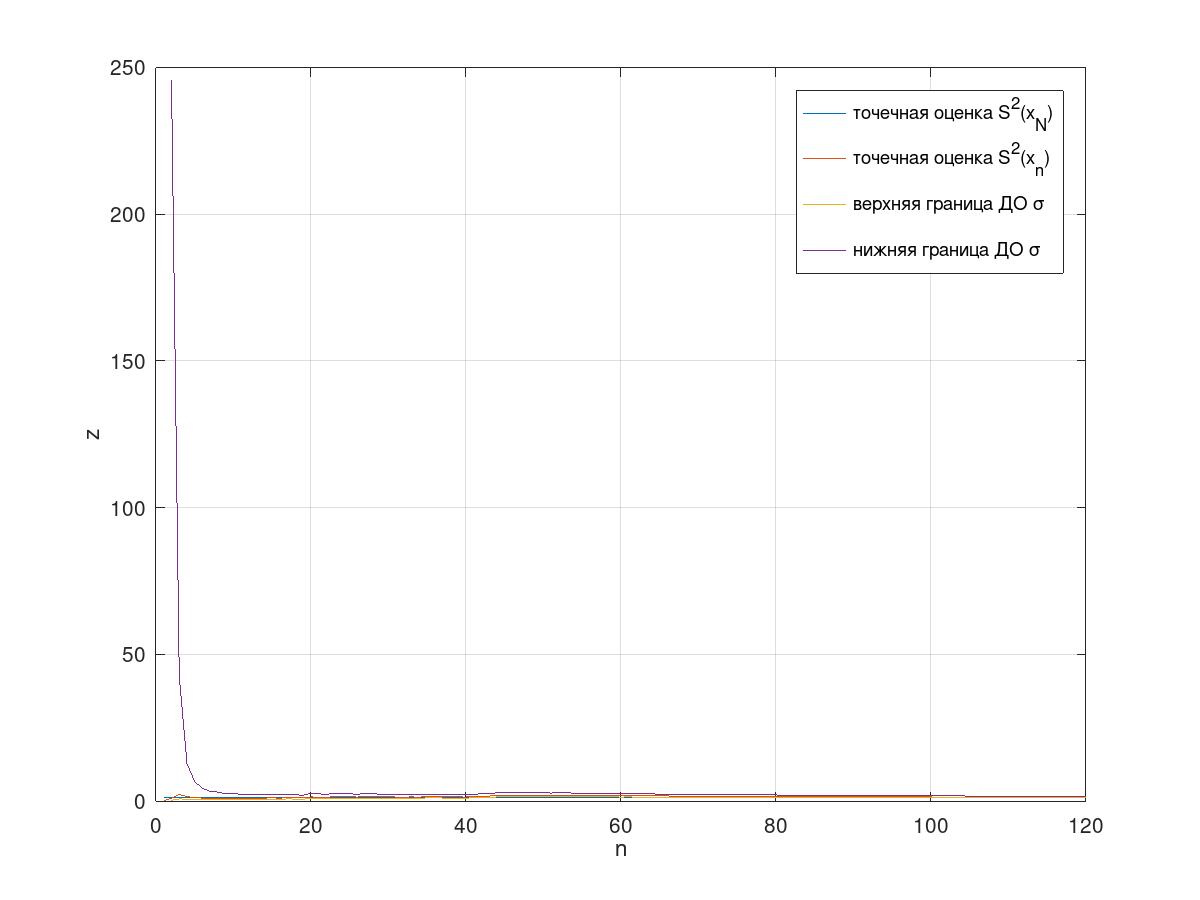
\includegraphics[scale=0.4]{assets/g2-1.jpg}
	\caption{Прямая $z=\hat S^2 (\vec x_N)$ и графики функций $z= S^2 (\vec x_n), z= \underline \sigma^2 (\vec x_n), z =\overline \sigma^2 (\vec x_n)$ как функций объема n выборки, где n изменяется от 1 до N.}
\end{figure}

\begin{figure}[H]
	\centering
	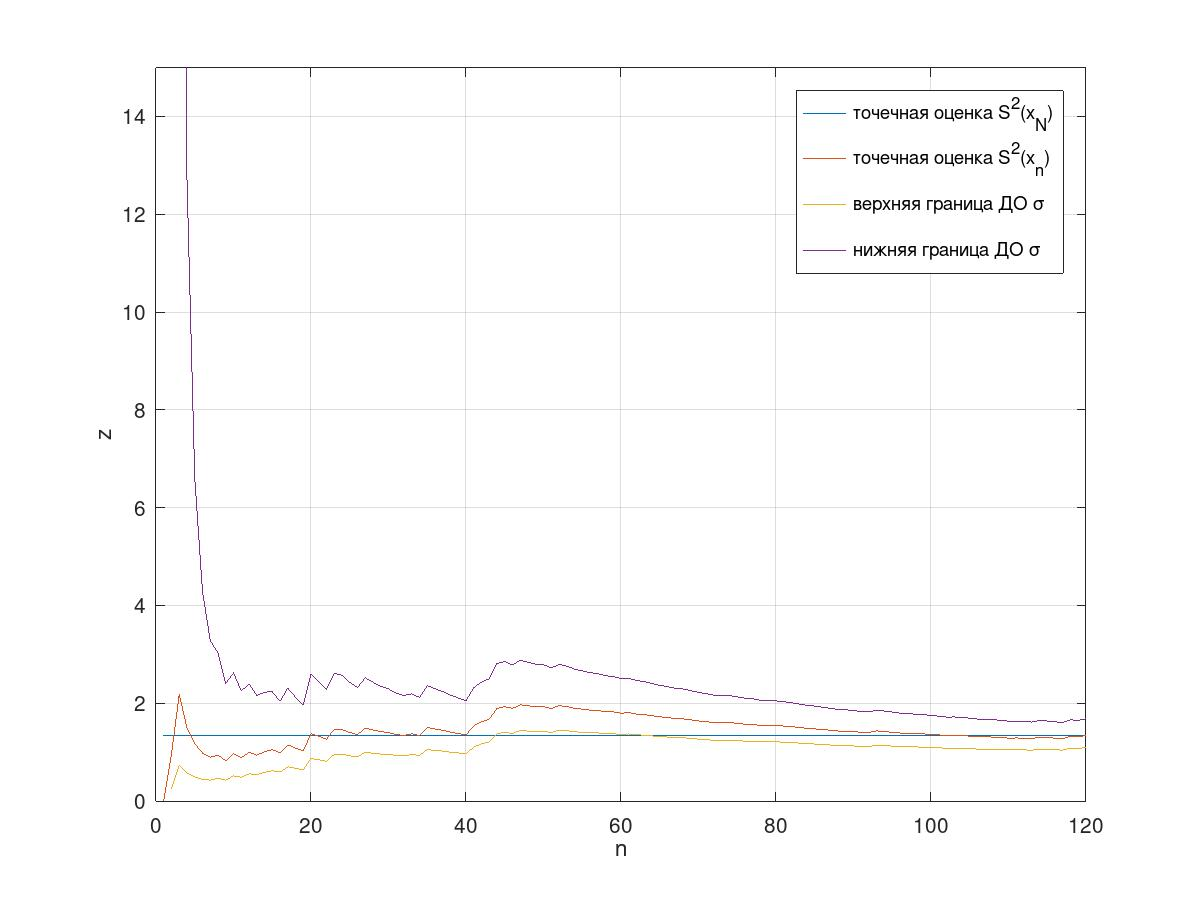
\includegraphics[scale=0.4]{assets/g2-2.jpg}
	\caption{Прямая $z=\hat S^2 (\vec x_N)$ и графики функций $z= S^2 (\vec x_n), z= \underline \sigma^2 (\vec x_n), z =\overline \sigma^2 (\vec x_n)$ как функций объема n выборки, где n изменяется от 1 до N.}
\end{figure}
